\documentclass[aps,pra,notitlepage,amsmath,amssymb,letterpaper,12pt]{revtex4-1}
\usepackage{amsthm}
\usepackage{graphicx}
%  Above uses the Americal Physical Society template for Physical Review A
%  as a reasonable and fully-featured default template
 
%  Below define helpful commands to set up problem environments easily
\newenvironment{problem}[2][Problem]{\begin{trivlist}
\item[\hskip \labelsep {\bfseries #1}\hskip \labelsep {\bfseries #2.}]}{\end{trivlist}}
\newenvironment{solution}{\begin{proof}[Solution]}{\end{proof}}
 
% --------------------------------------------------------------
%                   Document Begins Here
% --------------------------------------------------------------
 
\begin{document}
\begin{abstract}
\textbf{Abstract:} In this document we will discuss the definition of the derivative.
\end{abstract}
 
\title{Derivative}
\author{Chelsea Parlett-Pelleriti, Chris Watkins}
\affiliation{CS510, Schmid College of Science and Technology, Chapman University}
\date{\today}

\maketitle

\section{What are derivatives?} % Specify main sections this way

% x.yz is the problem number
\begin{problem}{1} 
The Definition of a Derivative
\end{problem}
 
\begin{solution} %You can also use proof in place of solution
A derivative is the rate of change at a single point on a function $f(x)$ 
\begin{align}
f'(x) = \lim_{x \rightarrow 0} \frac{f(x+h)-f(x)}{x+h}
\end{align}
% Use align environments for equations. The \\ is a newline character. The & is the alignment character.
% Using align* or \nonumber on each line removes equation numbers
\end{solution}

%\subsection{Subsection Title Here} % Specify subsections and subsubsections this way


\begin{figure}[h!] % h forces the figure to be placed here, in the text
  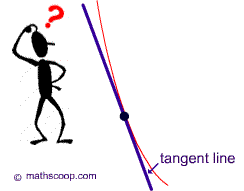
\includegraphics[width=0.4\textwidth]{1.png}  % if pdflatex is used, jpg, pdf, and png are permitted
  \caption{derivatives may be confusing at first, but keep going  http://www.mathscoop.com/calculus/derivatives/}
  \label{fig:figlabel}
\end{figure}

 
% Repeat as needed
 
\end{document}